\chapter{陆生植物的生活史与繁殖}\label{ch:b2:plant-life-cycles}

墙上那丛绿色的\omterm{def:b2:plant-life-cycles:moss}{苔藓}是一株植物；
春天从其上抽出的褐色茎秆，每根都顶着一个孢蒴，是另一株植物——
一个不同的个体，染色体数目是前者的两倍，
从前者长出，并依附于前者生活。\omterm{def:b2:plant-life-cycles:fern}{蕨类}的叶片背面带有孢子，
但这些孢子并不长成\omterm{def:b2:plant-life-cycles:fern}{蕨类}植物：它们
长成一片心形的绿色鳞片，宽仅几毫米，
精子和卵即在其中产生，新的\omterm{def:b2:plant-life-cycles:fern}{蕨类}植株正是从这片鳞片上
长出。所有陆生植物都以这种方式，在
两个个体之间交替：一为\omterm{def:b2:meiosis-heredity:meiosis}{单倍体}，一为\omterm{def:b2:meiosis-heredity:meiosis}{二倍体}。本章循着
这一交替过程，从藻类讲到种子，并说明一系列
变化——\omterm{def:b2:meiosis-heredity:meiosis}{单倍体}植株的缩小、\omterm{def:b2:plant-life-cycles:heterospory}{花粉}的出现、
\omterm{def:b2:plant-life-cycles:heterospory}{胚珠}的包被、种子的形成——如何使生殖摆脱了对水的依赖，
使植物得以覆盖大陆。

\section{三种生活史类型}

\begin{definition}[单倍体型、二倍体型与单倍–二倍体型生活史]\label{def:b2:plant-life-cycles:cycles}
\index{生活史}\index{世代交替}\index{配子体}\index{孢子体}
每个有性生活史中都有一次\emph{受精}，使染色体数目加倍，
也都有一次\emph{\omterm{def:b2:meiosis-heredity:meiosis}{减数分裂}}，使染色体数目减半；
各类生活史的不同之处，在于两者之间发生的事情。在
\emph{\omterm{def:b2:meiosis-heredity:meiosis}{单倍体}型}生活史中，合子是唯一的\omterm{def:b2:meiosis-heredity:meiosis}{二倍体}细胞，
并立即进行\omterm{def:b2:meiosis-heredity:meiosis}{减数分裂}；生物体为\omterm{def:b2:meiosis-heredity:meiosis}{单倍体}，其配子通过
有丝分裂产生（\emph{Chlamydomonas}、许多藻类和真菌）。
在\emph{\omterm{def:b2:meiosis-heredity:meiosis}{二倍体}型}生活史中，\omterm{def:b2:meiosis-heredity:meiosis}{减数分裂}直接产生配子，
配子是唯一的\omterm{def:b2:meiosis-heredity:meiosis}{单倍体}细胞，生物体为\omterm{def:b2:meiosis-heredity:meiosis}{二倍体}，
（动物、褐藻\emph{Fucus}）。在\emph{单倍–\omterm{def:b2:meiosis-heredity:meiosis}{二倍体}型}
生活史中，\omterm{def:b2:meiosis-heredity:meiosis}{减数分裂}产生\emph{孢子}，孢子通过有丝分裂
发育为\omterm{def:b2:meiosis-heredity:meiosis}{单倍体}生物体，即\emph{配子体}，配子体通过
有丝分裂产生配子；合子通过有丝分裂发育为\omterm{def:b2:meiosis-heredity:meiosis}{二倍体}生物体，即
\emph{孢子体}，孢子体通过\omterm{def:b2:meiosis-heredity:meiosis}{减数分裂}产生孢子。两个多细胞
个体交替出现——即\emph{世代交替}——
这正是所有陆生植物以及许多藻类的生活史。
\end{definition}

\begin{omfigure}
\begin{tikzpicture}[every node/.style={font=\scriptsize}, >=stealth]
  \foreach \dx/\title/\hap/\dip in {0/{单倍体型（\emph{衣藻}）}/{单倍体生物（$n$）}/{合子（$2n$）}, 5.2/{二倍体型（动物）}/{配子（$n$）}/{二倍体生物（$2n$）}, 10.4/{单双倍体型（植物）}/{配子体（$n$）}/{孢子体（$2n$）}} {
    \begin{scope}[xshift=\dx cm]
      \node[anchor=south, font=\scriptsize\bfseries] at (2,2.5) {\title};
      \draw[thick, omDef, ->] (0.6,0.4) arc (200:340:1.5 and 1.0);
      \draw[thick, omThm, ->] (3.4,1.4) arc (20:160:1.5 and 1.0);
      \node[omDef, anchor=north] at (2,-0.3) {\hap};
      \node[omThm, anchor=south] at (2,2.05) {\dip};
      \node[anchor=south west] at (3.4,1.05) {受精};
      \node[anchor=north east] at (0.55,0.75) {减数分裂};
    \end{scope}
  }
  % emphasise the dominant phase by thickness of the arcs: draw thicker arcs
  \draw[line width=2.4pt, omDef, ->] (0.6,0.4) arc (200:340:1.5 and 1.0);
  \draw[line width=2.4pt, omThm, ->] (5.2+3.4,1.4) arc (20:160:1.5 and 1.0);
  \draw[line width=2.4pt, omDef, ->] (10.4+0.6,0.4) arc (200:340:1.5 and 1.0);
  \draw[line width=2.4pt, omThm, ->] (10.4+3.4,1.4) arc (20:160:1.5 and 1.0);
\end{tikzpicture}

{\small 三种\omterm{def:b2:plant-life-cycles:cycles}{生活史}。蓝色：\omterm{def:b2:meiosis-heredity:meiosis}{单倍体}时期；红色：\omterm{def:b2:meiosis-heredity:meiosis}{二倍体}
时期；粗弧线代表多细胞个体。每种\omterm{def:b2:plant-life-cycles:cycles}{生活史}
都恰好经过一次\omterm{def:b2:meiosis-heredity:meiosis}{减数分裂}和一次受精；它们
的区别在于是哪一个时期（或两个时期）发育成生物体。}
\end{omfigure}

\begin{proposition}[世代交替的含义]\label{prop:b2:plant-life-cycles:alternation}
在陆生植物中，两个世代是两个生物体，而非同一生物的两个阶段：
\omterm{def:b2:plant-life-cycles:cycles}{配子体}与\omterm{def:b2:plant-life-cycles:cycles}{孢子体}的基因组不同（分别为\omterm{def:b2:meiosis-heredity:meiosis}{单倍体}和\omterm{def:b2:meiosis-heredity:meiosis}{二倍体}），
身体结构也不同，大小常相差数个数量级，
且二者都由单个细胞（孢子或合子）经有丝分裂发育而成。
\omterm{def:b2:plant-life-cycles:cycles}{配子体}在多细胞器官中产生配子：
\emph{\omterm{def:b2:plant-life-cycles:moss}{精子器}}（产生精子）与\emph{\omterm{def:b2:plant-life-cycles:moss}{颈卵器}}
（每个\omterm{def:b2:plant-life-cycles:moss}{颈卵器}内含一个卵，卵位于瓶状结构中，精子沿其颈部游入）；
\omterm{def:b2:plant-life-cycles:cycles}{孢子体}在\emph{\omterm{def:b2:plant-life-cycles:fern}{孢子囊}}中产生孢子。跨越整个陆生植物类群，
两个世代的主次关系发生了变化：\omterm{def:b2:plant-life-cycles:moss}{苔藓}中\omterm{def:b2:plant-life-cycles:cycles}{配子体}即植物本体，
\omterm{def:b2:plant-life-cycles:cycles}{孢子体}则是依附其上的茎柄；\omterm{def:b2:plant-life-cycles:fern}{蕨类}中\omterm{def:b2:plant-life-cycles:cycles}{孢子体}即植物本体，
\omterm{def:b2:plant-life-cycles:cycles}{配子体}则是独立生活的小片状体；种子植物中，
\omterm{def:b2:plant-life-cycles:cycles}{配子体}退化为隐藏在\omterm{def:b2:plant-life-cycles:cycles}{孢子体}组织内的几个细胞，
即\omterm{def:b2:plant-life-cycles:heterospory}{花粉}粒和\omterm{def:b2:plant-life-cycles:heterospory}{胚珠}中的内容物。
\end{proposition}
\begin{proof}[证据]
霍夫迈斯特（1851 年）使\omterm{def:b2:plant-life-cycles:moss}{苔藓}、\omterm{def:b2:plant-life-cycles:fern}{蕨类}、
木贼和石松的孢子萌发，追踪它们产生的小绿体的发育，
并在其上发现了\omterm{def:b2:plant-life-cycles:moss}{精子器}和\omterm{def:b2:plant-life-cycles:moss}{颈卵器}，
还观察到胚从\omterm{def:b2:plant-life-cycles:moss}{颈卵器}内的受精卵发育为
产孢植物。他接着指出，\omterm{prop:b2:plant-life-cycles:conifer}{针叶树}的\omterm{def:b2:plant-life-cycles:heterospory}{胚珠}含有相同结构，
只是已经退化——
\omterm{def:b2:plant-life-cycles:moss}{颈卵器}位于一种残留\omterm{def:b2:plant-life-cycles:cycles}{配子体}组织之内——
由此可见，\omterm{def:b2:plant-life-cycles:moss}{苔藓}、\omterm{def:b2:plant-life-cycles:fern}{蕨类}与种子植物是同一系列，具有同一\omterm{def:b2:plant-life-cycles:cycles}{生活史}。
用以解释两个世代的染色体数目的工作（斯特拉斯布格尔，
1894 年）则晚了四十年才出现。
\end{proof}

\section{苔藓：配子体即植物本体}

\begin{definition}[苔藓的生活史]\label{def:b2:plant-life-cycles:moss}
\index{苔藓}\index{原丝体}\index{颈卵器}\index{精子器}
苔藓的\emph{孢子}萌发成一条分枝的绿色丝状体，即
\emph{原丝体}，其上的芽发育为有叶的枝条——即
\emph{\omterm{def:b2:plant-life-cycles:cycles}{配子体}}，高仅数厘米，没有真正的根、
木质部或韧皮部，靠假根固定，并经由其
整个表面吸收水分。枝条顶端着生\emph{精子器}，
释放双鞭毛精子，进入雨水或露水形成的水膜，
\emph{颈卵器}，每个内含一枚卵，卵位于颈部底部；
精子最多游动数厘米，受化学引诱物引导，
并就地使卵受精。合子发育为
\emph{\omterm{def:b2:plant-life-cycles:cycles}{孢子体}}：足部嵌入\omterm{def:b2:plant-life-cycles:cycles}{配子体}中，有一根
\emph{蒴柄}，以及一个\emph{孢蒴}，孢蒴内\omterm{def:b2:meiosis-heredity:meiosis}{减数分裂}产生数以万计的
孢子，孢子经由一圈吸湿齿释放，
这些齿在干燥空气中张开。\omterm{def:b2:plant-life-cycles:cycles}{孢子体}自身能进行少量光合作用，但
须由\omterm{def:b2:plant-life-cycles:cycles}{配子体}通过其足部供给养分，从不单独生活。
\end{definition}

\begin{omfigure}
\begin{tikzpicture}[every node/.style={font=\scriptsize}, >=stealth]
  \node[draw, rounded corners, fill=omDef!12, align=center] (spore) at (0,3) {孢子 ($n$)};
  \node[draw, rounded corners, fill=omDef!12, align=center] (proto) at (3.2,3) {原丝体};
  \node[draw, rounded corners, fill=omDef!12, align=center] (gam) at (6.6,3) {叶状配子体 ($n$)\\精子器和颈卵器};
  \node[draw, rounded corners, fill=omDef!12, align=center] (gametes) at (11.2,3) {精子和卵 ($n$)};
  \node[draw, rounded corners, fill=omThm!12, align=center] (zyg) at (11.2,0.8) {合子 ($2n$)};
  \node[draw, rounded corners, fill=omThm!12, align=center] (sporo) at (6.6,0.8) {孢子体 ($2n$)\\足部、蒴柄、孢蒴};
  \node[draw, rounded corners, fill=omThm!12, align=center] (cap) at (2.4,0.8) {孢蒴中的减数分裂};
  \draw[->, thick] (spore) -- (proto) node[midway, above] {有丝分裂};
  \draw[->, thick] (proto) -- (gam);
  \draw[->, thick] (gam) -- (gametes) node[midway, above] {有丝分裂};
  \draw[->, thick] (gametes) -- (zyg) node[pos=0.3, right, align=left] {受精 \\在水膜中};
  \draw[->, thick] (zyg) -- (sporo) node[midway, above] {有丝分裂};
  \draw[->, thick] (sporo) -- (cap);
  \draw[->, thick] (cap) -| (spore) ;
  \node[omDef, anchor=west] at (-1.9,3.9) {单倍体};
  \node[omThm, anchor=west] at (-1.9,-0.1) {二倍体};
  \draw[gray, dashed] (-1.9,1.9) -- (13.2,1.9);
\end{tikzpicture}

{\small \omterm{def:b2:plant-life-cycles:moss}{苔藓}生命周期。叶状植株即\omterm{def:b2:meiosis-heredity:meiosis}{单倍体}\omterm{def:b2:plant-life-cycles:cycles}{配子体}；
\omterm{def:b2:plant-life-cycles:cycles}{孢子体}是长在其上、由它供养的蒴柄与孢蒴，
并通过\omterm{def:b2:meiosis-heredity:meiosis}{减数分裂}产生孢子。}
\end{omfigure}

\begin{omfigure}
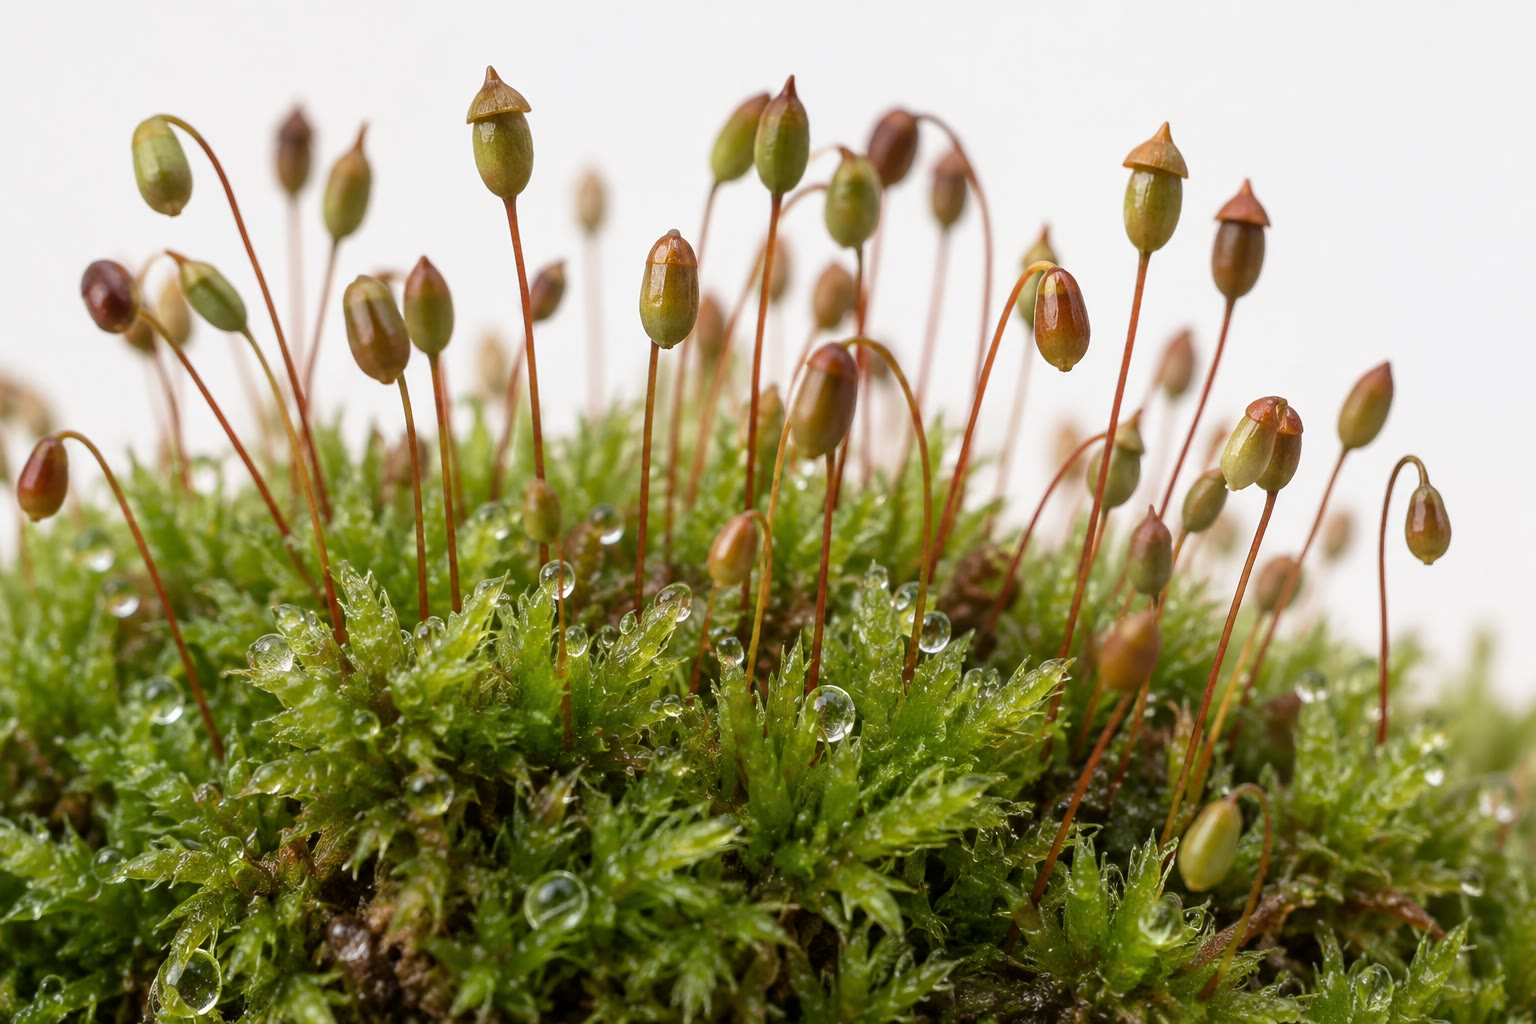
\includegraphics[width=0.6\linewidth]{images/book4/ai/b4-05-moss-sporophytes.jpg}

{\small 春季的一片\omterm{def:b2:plant-life-cycles:moss}{苔藓}垫：绿色枝条是
\omterm{def:b2:plant-life-cycles:cycles}{配子体}，每根带孢蒴的红色蒴柄都是
由受精卵发育而来的\omterm{def:b2:plant-life-cycles:cycles}{孢子体}，仍与产生卵的
枝条相连。}
\end{omfigure}

\begin{example}[游动精子的代价]\label{ex:b2:plant-life-cycles:sperm}
\omterm{def:b2:plant-life-cycles:moss}{苔藓}精子以约 \qty{100}{\micro m/s} 的速度游动；要到达一个
相距 \qty{2}{cm} 的\omterm{def:b2:plant-life-cycles:moss}{颈卵器}，需要 \qty{200}{s} 的连续
水膜——一场溅起的雨水，或一层厚露。受精因此
只能发生在潮湿天气和短距离之内；大多数
\omterm{def:b2:plant-life-cycles:moss}{苔藓}、\omterm{def:b2:plant-life-cycles:fern}{蕨类}及其近缘类群生活在潮湿处，或在
雨季繁殖；某些\omterm{def:b2:plant-life-cycles:moss}{苔藓}的\omterm{def:b2:plant-life-cycles:moss}{精子器}位于溅水杯中，
其形状可将雨滴溅出，并将所携精子送出半米。
种子植物摆脱了这种依赖。
\end{example}

\section{蕨类：孢子体即植株}

\begin{definition}[蕨类的生命周期]\label{def:b2:plant-life-cycles:fern}
\index{蕨类}\index{原叶体}\index{孢子囊群}\index{孢子囊}
蕨类即\emph{\omterm{def:b2:plant-life-cycles:cycles}{孢子体}}：具有根状茎、根、木质部和
韧皮部，以及叶片。在能育叶片背面，成簇的
\emph{孢子囊}（\emph{孢子囊群}，常位于保护性瓣膜下）各
经\omterm{def:b2:meiosis-heredity:meiosis}{减数分裂}产生 64 个孢子，靠干燥的
厚壁细胞环的突然弹开将其抛射出去。落在湿润土壤上的孢子
长成\emph{原叶体}：一种心形绿色\omterm{def:b2:plant-life-cycles:cycles}{配子体}，直径约
数毫米，仅一个细胞厚，具有假根，自由生活
数周。其背面着生\omterm{def:b2:plant-life-cycles:moss}{精子器}和\omterm{def:b2:plant-life-cycles:moss}{颈卵器}；精子
在土壤水膜中游向卵细胞；合子发育为幼嫩的
\omterm{def:b2:plant-life-cycles:cycles}{孢子体}，先从原叶体获取最初的养分，之后
长出根，原叶体随之死亡。两个世代都
独立，但并不对等：\omterm{def:b2:plant-life-cycles:cycles}{孢子体}可存活数十年，
可高达数米；\omterm{def:b2:plant-life-cycles:cycles}{配子体}只存活数周，大小仅数毫米。
\end{definition}

\begin{omfigure}
\begin{tikzpicture}[every node/.style={font=\scriptsize}, >=stealth]
  \node[draw, rounded corners, fill=omThm!12, align=center] (fern) at (0,3) {蕨类植株，即孢子体 ($2n$)\\根、根状茎、叶片};
  \node[draw, rounded corners, fill=omThm!12, align=center] (sor) at (5.4,3) {孢子囊群中的孢子囊 \\（位于叶片背面）};
  \node[draw, rounded corners, fill=omDef!12, align=center] (spore) at (10.4,3) {孢子 ($n$)\\每个孢子囊 64 个};
  \node[draw, rounded corners, fill=omDef!12, align=center] (pro) at (10.4,0.6) {原叶体 ($n$)\\自由生活，毫米级 \\精子器、颈卵器};
  \node[draw, rounded corners, fill=omDef!12, align=center] (gam) at (5.4,0.6) {精子和卵 ($n$)};
  \node[draw, rounded corners, fill=omThm!12, align=center] (zyg) at (0,0.6) {合子 ($2n$)，随后 \\幼龄孢子体 \\生长于原叶体上};
  \draw[->, thick] (fern) -- (sor);
  \draw[->, thick] (sor) -- (spore) node[midway, above] {减数分裂};
  \draw[->, thick] (spore) -- (pro) node[midway, right] {有丝分裂};
  \draw[->, thick] (pro) -- (gam) node[midway, above] {有丝分裂};
  \draw[->, thick] (gam) -- (zyg) node[midway, above, align=center] {受精 \\（游动的精子）};
  \draw[->, thick] (zyg) -- (fern) node[midway, right] {有丝分裂};
  \draw[gray, dashed] (7.9,-0.5) -- (7.9,4.0);
  \node[omThm, anchor=south] at (2.7,3.9) {二倍体世代};
  \node[omDef, anchor=south] at (10.4,3.9) {单倍体世代};
\end{tikzpicture}

{\small \omterm{def:b2:plant-life-cycles:fern}{蕨类}生命周期。我们通常所说的\omterm{def:b2:plant-life-cycles:fern}{蕨类}植株是\omterm{def:b2:meiosis-heredity:meiosis}{二倍体}
\omterm{def:b2:plant-life-cycles:cycles}{孢子体}；\omterm{def:b2:meiosis-heredity:meiosis}{单倍体}\omterm{def:b2:plant-life-cycles:cycles}{配子体}是短暂存在的\omterm{def:b2:plant-life-cycles:fern}{原叶体}，
精子在其上游向卵细胞。}
\end{omfigure}

\begin{omfigure}
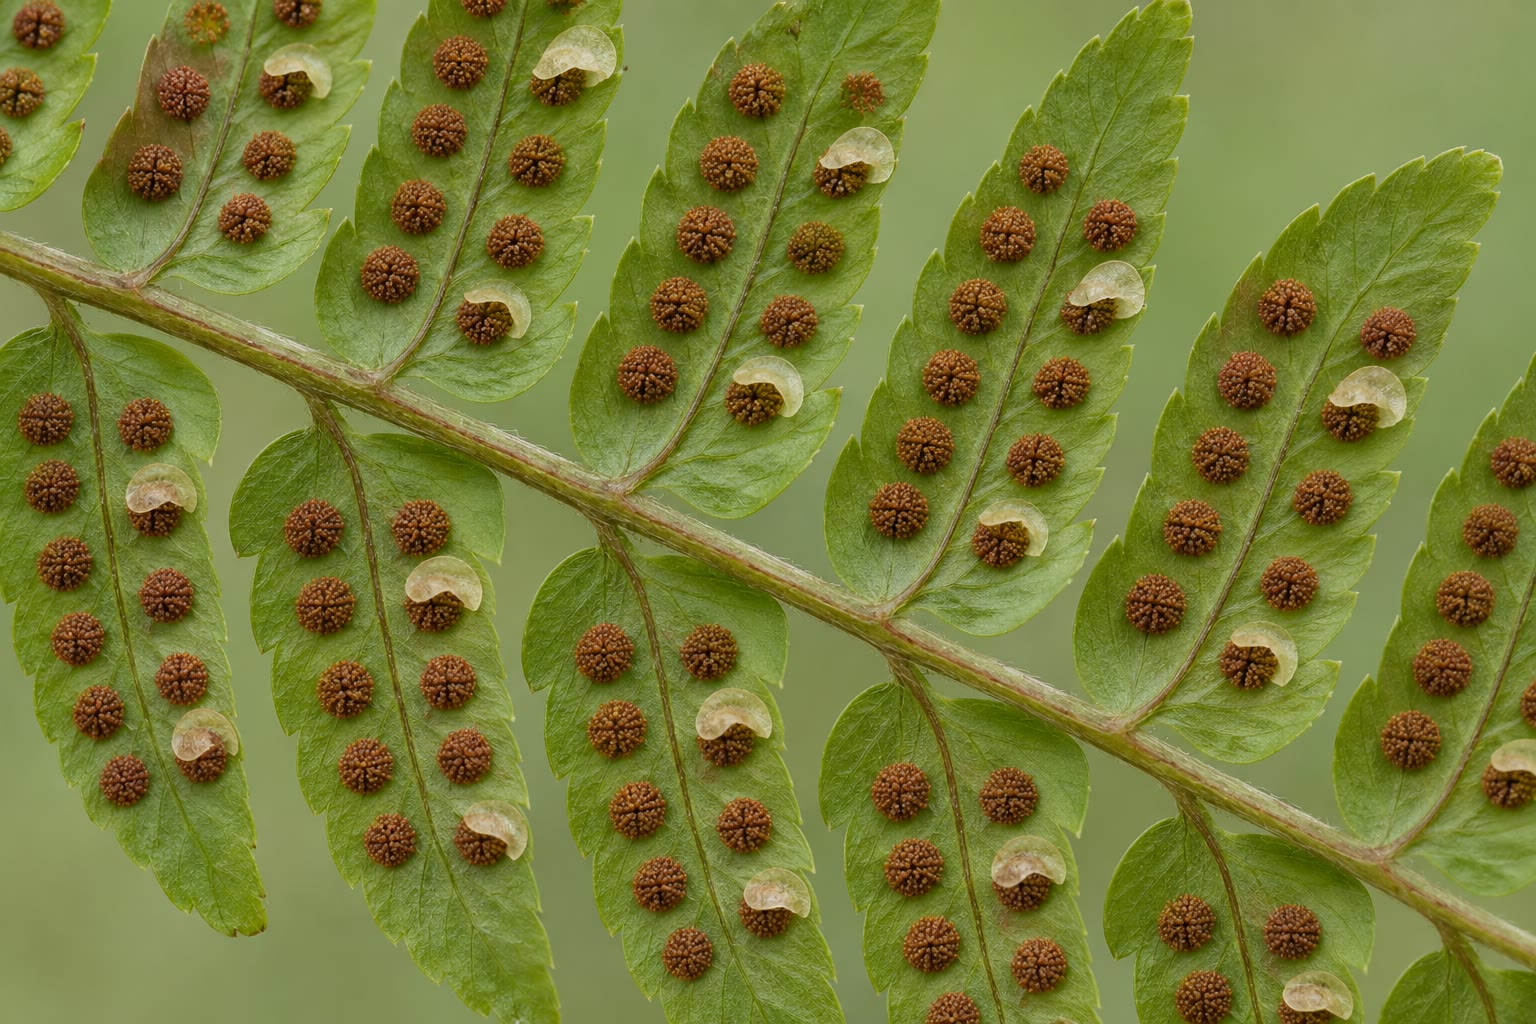
\includegraphics[width=0.6\linewidth]{images/book4/ai/b4-05-fern-sori.jpg}

{\small 能育\omterm{def:b2:plant-life-cycles:fern}{蕨类}叶片的背面：每个褐色圆点是一个
\omterm{def:b2:plant-life-cycles:fern}{孢子囊群}，即一簇\omterm{def:b2:plant-life-cycles:fern}{孢子囊}，其中一些仍被保护它们的瓣膜覆盖，
直至成熟。}
\end{omfigure}

\begin{theorem}[孢子的扩散]\label{thm:b2:plant-life-cycles:dispersal}
\index{孢子扩散}
设半径为 $r$、密度为 $\rho_s$ 的孢子在高度 $h$ 处释放，
进入速度为 $u$ 的水平风中，以斯托克斯终端
速度 $v_s = 2r^2(\rho_s - \rho_{\text{空气}})g/9\eta_{\text{空气}}$ 下落，
并在分层静止的空气中落下，落点距
\[
x = \frac{u\,h}{v_s}
\]
植株的距离。一枚\omterm{def:b2:plant-life-cycles:fern}{蕨类}孢子，半径为 \qty{15}{\micro m}，
密度为 \qty{1100}{kg/m^3}（$\eta_{\text{空气}} = \qty{1.8e-5}{Pa.s}$），
以 \qty{3}{cm/s} 下落；从 \qty{0.5}{m} 高的叶片释放，
在风速 \qty{2}{m/s} 的风中约飘移 \qty{30}{m}；在
大风天的湍流空气中，部分孢子被抬升到远高于
释放高度之处，少数孢子可飘移数百千米——这正是
海洋岛屿\omterm{def:b2:plant-life-cycles:fern}{蕨类}区系丰富而种子植物区系
贫乏的原因。
\end{theorem}
\begin{proof}
下落时间为 $h/v_s$（孢子在
数微秒内即达终端速度），其间风将其带走 $u\,h/v_s$。
终端速度由平衡斯托克斯阻力 $6\pi\eta r
v_s$ 与重力减去浮力 $\tfrac43\pi r^3(\rho_s -
\rho_{\text{空气}})g$，如\cref{ch:b2:unicellular-diversity}中所述。
\end{proof}

\section{种子植物：配子体是隐蔽的}

\begin{definition}[异型孢子性、花粉、胚珠]\label{def:b2:plant-life-cycles:heterospory}
\index{异型孢子性}\index{花粉}\index{胚珠}\index{小孢子}\index{大孢子}
\omterm{def:b2:plant-life-cycles:moss}{苔藓}和大多数\omterm{def:b2:plant-life-cycles:fern}{蕨类}为\emph{同型孢子}：只产生一种孢子，
由它发育出一种同时带有雌雄两性的\omterm{def:b2:plant-life-cycles:cycles}{配子体}。种子植物（以及少数
\omterm{def:b2:plant-life-cycles:fern}{蕨类}和石松类）为\emph{异型孢子}植物：\emph{小孢子}，
数量多而个体小，发育为雄\omterm{def:b2:plant-life-cycles:cycles}{配子体}；\emph{大孢子}个大而数少，
发育为雌\omterm{def:b2:plant-life-cycles:cycles}{配子体}。在种子植物中，两者都退化到
几乎只剩最简结构，二者都不能独自脱离\omterm{def:b2:plant-life-cycles:cycles}{孢子体}的组织。
雄\omterm{def:b2:plant-life-cycles:cycles}{配子体}即\emph{花粉粒}：一个小孢子
在壁内分裂两至三次，借风或动物
传送到雌性器官，在那里长出\emph{花粉管}，
并送出精子，无需水。雌\omterm{def:b2:plant-life-cycles:cycles}{配子体}
在大\omterm{def:b2:plant-life-cycles:fern}{孢子囊}内发育；大\omterm{def:b2:plant-life-cycles:fern}{孢子囊}仍留在亲本上，
由一层或两层带孔的\emph{珠被}包裹，此孔即
\emph{珠孔}：整个结构称为\emph{胚珠}。受精后
胚珠发育为\emph{种子}：一个幼小\omterm{def:b2:plant-life-cycles:cycles}{孢子体}（胚），
一份食物储备，以及由珠被形成的种皮，
处于休眠，直到条件适宜为止。
\end{definition}

\begin{omfigure}
\begin{tikzpicture}[every node/.style={font=\scriptsize}]
  % ovule in section
  \draw[thick, fill=omExo!25] (0,0) ellipse (1.6 and 2.2);
  \draw[thick, fill=omExo!10] (0,0) ellipse (1.25 and 1.85);
  \draw[thick, fill=white] (0,-0.15) ellipse (0.8 and 1.3);
  \draw[thick, fill=omDef!25] (0,0.6) ellipse (0.45 and 0.55);
  \fill[omDef!80!black] (0,0.75) circle (0.12);
  % micropyle: gap at top
  \fill[white] (-0.35,1.7) rectangle (0.35,2.35);
  \draw[thick] (-0.35,1.7) -- (-0.35,2.2); \draw[thick] (0.35,1.7) -- (0.35,2.2);
  \draw[thick] (-0.35,2.2) arc (180:90:0.1) ; \draw[thick] (0.35,2.2) arc (0:90:0.1);
  % pollen grain and tube
  \draw[thick, fill=omProp!40] (0.9,3.0) circle (0.22);
  \draw[thick, omProp] (0.75,2.85) .. controls (0.2,2.6) and (0.05,2.0) .. (0.05,1.25);
  % stalk
  \draw[thick] (0,-2.2) -- (0,-2.8);
  % labels
  \draw (1.45,-0.9) -- (2.6,-0.9) node[right] {珠被};
  \draw (1.0,-0.6) -- (2.6,-1.5) node[right] {大孢子囊（珠心）};
  \draw (0.55,-1.0) -- (2.6,-2.1) node[right, align=left] {雌配子体 \\\\（由一个大孢子发育而来）};
  \draw (0.35,0.45) -- (2.6,0.3) node[right] {颈卵器};
  \draw (0.1,0.78) -- (2.6,1.0) node[right] {卵};
  \draw (0.35,2.0) -- (2.6,2.0) node[right] {珠孔};
  \draw (1.1,3.0) -- (2.6,3.0) node[right] {花粉粒和花粉管};
  \node[right] at (0.1,-2.6) {柄};
\end{tikzpicture}

{\small 裸子植物\omterm{def:b2:plant-life-cycles:heterospory}{胚珠}的纵切面。雌\omterm{def:b2:plant-life-cycles:cycles}{配子体}由
大\omterm{def:b2:plant-life-cycles:fern}{孢子囊}内的单个\omterm{def:b2:plant-life-cycles:heterospory}{大孢子}发育而成，被一层带孔的
珠被包裹；\omterm{def:b2:plant-life-cycles:heterospory}{花粉}粒落在珠孔处，
长出\omterm{def:b2:plant-life-cycles:heterospory}{花粉}管通向卵。受精后，整体发育为
种子。}
\end{omfigure}

\begin{proposition}[针叶树的生活史]\label{prop:b2:plant-life-cycles:conifer}
\index{针叶树}\index{球果}\index{种子}
松树有两种\omterm{prop:b2:plant-life-cycles:conifer}{球果}。较小的\emph{雄\omterm{prop:b2:plant-life-cycles:conifer}{球果}}，
春季成簇着生，内有小\omterm{def:b2:plant-life-cycles:fern}{孢子囊}，其中经\omterm{def:b2:meiosis-heredity:meiosis}{减数分裂}产生\omterm{def:b2:plant-life-cycles:heterospory}{小孢子}；
每个\omterm{def:b2:plant-life-cycles:heterospory}{小孢子}分裂为一个四细胞\omterm{def:b2:plant-life-cycles:heterospory}{花粉}粒，带有两个气囊，
数以百万计地被散入风中。\emph{雌\omterm{prop:b2:plant-life-cycles:conifer}{球果}}的每个鳞片上侧
着生两枚\omterm{def:b2:plant-life-cycles:heterospory}{胚珠}。被风吹入鳞片间的\omterm{def:b2:plant-life-cycles:heterospory}{花粉}
由一滴液体引至珠孔；雌\omterm{def:b2:plant-life-cycles:cycles}{配子体}
尚未发育，随后在次年内
由存活的单个\omterm{def:b2:plant-life-cycles:heterospory}{大孢子}发育为一团
约数千个细胞、带有两至三个\omterm{def:b2:plant-life-cycles:moss}{颈卵器}的组织；\omterm{def:b2:plant-life-cycles:heterospory}{花粉}管
缓慢穿过珠心，于授粉后十五个月
将一个精子送至卵。胚在
\omterm{def:b2:plant-life-cycles:cycles}{配子体}内发育，\omterm{def:b2:plant-life-cycles:cycles}{配子体}成为种子的食物储备；种子
带翅，于第二年秋季\omterm{prop:b2:plant-life-cycles:conifer}{球果}开裂时脱落。种子
需耗时数年，代价高昂；作为回报，种子以干燥状态散布，
能耐受冬季与干旱，并携带幼苗最初数周所需的
食物。
\end{proposition}

\begin{omfigure}
\begin{tikzpicture}[every node/.style={font=\scriptsize}, >=stealth]
  \draw[thick, ->] (0,0) -- (13.2,0);
  \foreach \x/\l in {0/{第 1 年春}, 4.4/{第 2 年春}, 8.8/{第 2 年秋}, 12.4/{}}
    \draw (\x,0.1) -- (\x,-0.1) node[below] {\l};
  \node[above, align=center, omProp] at (0.6,0.3) {传粉：\\花粉落在珠孔处};
  \node[above, align=center, omDef] at (3.0,1.2) {雌配子体由大孢子发育 \\（历时一年）};
  \draw[omDef, thick] (0.8,1.15) -- (5.2,1.15);
  \node[above, align=center, omThm] at (5.6,0.3) {受精：\\花粉管到达卵};
  \node[above, align=center, omThm] at (8.2,1.2) {胚在配子体内 \\发育};
  \draw[omThm, thick] (5.8,1.15) -- (10.4,1.15);
  \node[above, align=center] at (10.8,0.3) {球果开裂：\\带翅种子脱落};
\end{tikzpicture}

{\small 松树种子的时间线：第一年春季传粉，
受精在一年多以后，种子于第二年
秋季脱落——从\omterm{def:b2:plant-life-cycles:heterospory}{花粉}到种子约十八个月。}
\end{omfigure}

\begin{omfigure}
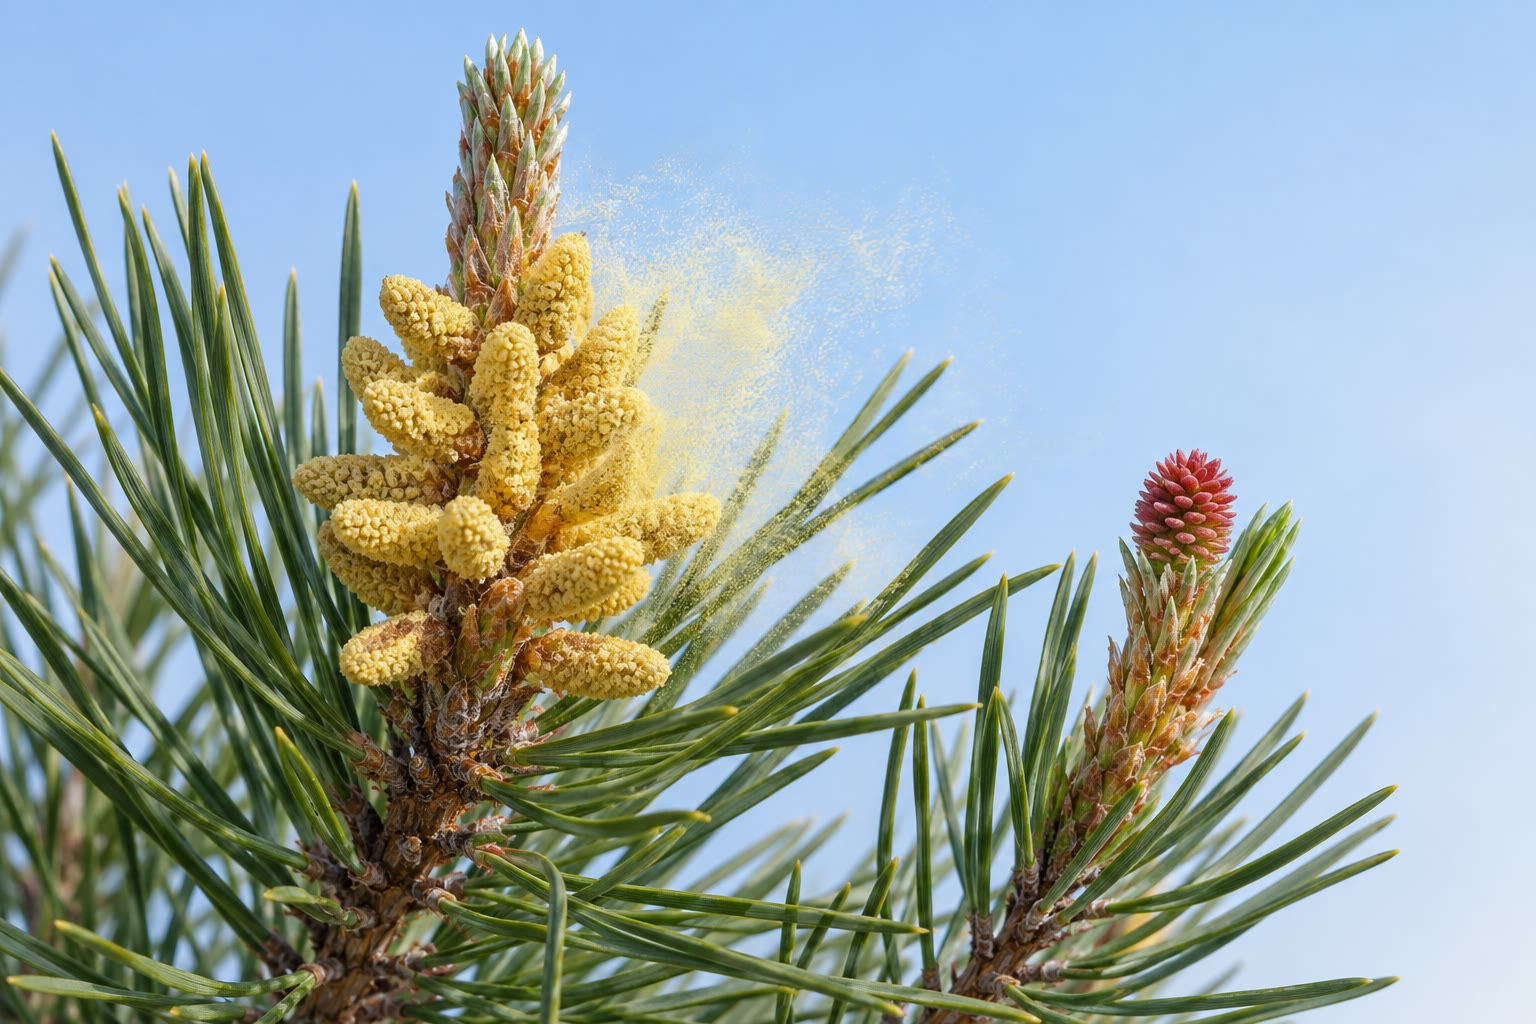
\includegraphics[width=0.6\linewidth]{images/book4/ai/b4-05-pine-cones.jpg}

{\small 春季的一段松枝：一簇黄色的雄\omterm{prop:b2:plant-life-cycles:conifer}{球果}
正在散粉，另一枝条顶端有一个小红色雌\omterm{prop:b2:plant-life-cycles:conifer}{球果}，
鳞片张开以承接\omterm{def:b2:plant-life-cycles:heterospory}{花粉}。}
\end{omfigure}

\begin{example}[风中的花粉]\label{ex:b2:plant-life-cycles:pollen}
一粒松树\omterm{def:b2:plant-life-cycles:heterospory}{花粉}粒，直径 \qty{50}{\micro m}，带有两个气囊，
以约 \qty{3}{cm/s} 的速度下落；一棵大树
一个季节释放约 $10^{11}$ 粒\omterm{def:b2:plant-life-cycles:heterospory}{花粉}，足以把池塘染成黄色。
某一粒\omterm{def:b2:plant-life-cycles:heterospory}{花粉}恰好落在特定\omterm{def:b2:plant-life-cycles:heterospory}{胚珠}上的机会极小，因此
这一策略只能靠数量取胜：风媒传粉每粒\omterm{def:b2:plant-life-cycles:heterospory}{花粉}成本低，
但耗用的\omterm{def:b2:plant-life-cycles:heterospory}{花粉}数量大，且只限于同种成片生长的植物
——如\omterm{prop:b2:plant-life-cycles:conifer}{针叶树}、禾草和栎树。开花植物
（\cref{ch:b2:angiosperm-reproduction}）找到了
借助动物递送\omterm{def:b2:plant-life-cycles:heterospory}{花粉}，每次一粒，准确送达目的地。
\end{example}

\section{陆生植物的趋势}

\begin{proposition}[四种趋势]\label{prop:b2:plant-life-cycles:trends}
\index{配子体的缩减}
从\omterm{def:b2:plant-life-cycles:moss}{苔藓}到\omterm{def:b2:plant-life-cycles:fern}{蕨类}再到种子植物：（1）\omterm{def:b2:plant-life-cycles:cycles}{孢子体}由依附的柄发育为
整株植物，\omterm{def:b2:plant-life-cycles:cycles}{配子体}则从整株缩小为鳞片状结构，最终只剩几个细胞；
（2）同型孢子让位于
异型孢子，雌\omterm{def:b2:plant-life-cycles:cycles}{配子体}留在亲本上；
（3）受精由精子在地表水中游动，转变为借助
\omterm{def:b2:plant-life-cycles:heterospory}{花粉}管完成，生殖因此不再依赖降雨；
（4）扩散单位由孢子——一个带有一天储备养分的单细胞——
转变为种子，即带有食物与种皮、能够等待的胚胎。
陆地上\omterm{def:b2:meiosis-heredity:meiosis}{二倍体}世代更占优势，原因在于\omterm{def:b2:meiosis-heredity:meiosis}{二倍体}
个体能掩盖\omterm{def:b2:meiosis-heredity:vocabulary}{隐性}\omterm{def:b2:genome-diversification:mutation}{突变}，并可借助维管系统长得更大、寿命更长，
而且高大\omterm{def:b2:plant-life-cycles:cycles}{孢子体}通过\omterm{def:b2:meiosis-heredity:meiosis}{减数分裂}产生的孢子，
比低矮\omterm{def:b2:plant-life-cycles:cycles}{配子体}上游动的配子传播得更远。
这一趋势延续到开花植物中，其中雌\omterm{def:b2:plant-life-cycles:cycles}{配子体}为七个细胞，
种子包裹在
果实之中。
\end{proposition}

\begin{example}[各类群比较]\label{ex:b2:plant-life-cycles:table}
\begin{center}
\small
\begin{tabular}{p{2.3cm}p{3.1cm}p{3.1cm}p{3.3cm}}
\hline
 & \omterm{def:b2:plant-life-cycles:moss}{苔藓} & \omterm{def:b2:plant-life-cycles:fern}{蕨类} & \omterm{prop:b2:plant-life-cycles:conifer}{针叶树} \\
\hline
优势世代 & \omterm{def:b2:plant-life-cycles:cycles}{配子体} & \omterm{def:b2:plant-life-cycles:cycles}{孢子体} & \omterm{def:b2:plant-life-cycles:cycles}{孢子体} \\
\omterm{def:b2:plant-life-cycles:cycles}{配子体} & 叶状枝，厘米级 & \omterm{def:b2:plant-life-cycles:fern}{原叶体}，毫米级，自由生活 & \omterm{def:b2:plant-life-cycles:heterospory}{花粉}粒（4 个细胞）；\omterm{def:b2:plant-life-cycles:heterospory}{胚珠}内容物（数千个细胞） \\
孢子 & 一种 & 一种 & \omterm{def:b2:plant-life-cycles:heterospory}{小孢子}、\omterm{def:b2:plant-life-cycles:heterospory}{大孢子} \\
受精 & 精子在水中游动 & 精子在水中游动 & \omterm{def:b2:plant-life-cycles:heterospory}{花粉}管 \\
扩散单位 & 孢子 & 孢子 & 种子 \\
维管组织 & 无 & 木质部、韧皮部 & 木质部、韧皮部、木材 \\
\hline
\end{tabular}
\end{center}
\end{example}

\section{练习}

\begin{exercise}[$\star$]\label{exo:b2:plant-life-cycles:1}
定义\omterm{def:b2:plant-life-cycles:cycles}{配子体}、\omterm{def:b2:plant-life-cycles:cycles}{孢子体}、孢子和配子，并说明这四者各由哪种
分裂（有丝分裂或\omterm{def:b2:meiosis-heredity:meiosis}{减数分裂}）产生。
\end{exercise}

\begin{exercise}[$\star$]\label{exo:b2:plant-life-cycles:2}
\omterm{def:b2:plant-life-cycles:fern}{蕨类}植物 \emph{Ophioglossum reticulatum} 的叶细胞中有 \num{1260}
条染色体。一个孢子、一个\omterm{def:b2:plant-life-cycles:fern}{原叶体}细胞、
一个精子、一个卵细胞和一个受精卵中分别有多少条染色体？
\end{exercise}

\begin{exercise}[$\star$]\label{exo:b2:plant-life-cycles:3}
\omterm{def:b2:plant-life-cycles:moss}{苔藓}的绿色垫状体属于哪一世代？带有孢蒴的褐色
柄呢？\omterm{def:b2:plant-life-cycles:fern}{蕨类}的羽叶呢？\omterm{def:b2:plant-life-cycles:fern}{原叶体}呢？\omterm{def:b2:plant-life-cycles:heterospory}{花粉}粒呢？
松树种子的食物储藏组织呢？松树种子的胚呢？
\end{exercise}

\begin{exercise}[$\star$]\label{exo:b2:plant-life-cycles:4}
写出三种\omterm{def:b2:plant-life-cycles:cycles}{生活史}类型，并各举一种生物为例。
各类\omterm{def:b2:plant-life-cycles:cycles}{生活史}中\omterm{def:b2:meiosis-heredity:meiosis}{减数分裂}分别发生在何处？
\end{exercise}

\begin{exercise}[$\star\star$]\label{exo:b2:plant-life-cycles:5}
\omterm{def:b2:plant-life-cycles:moss}{苔藓}精子以 \qty{100}{\micro m/s} 的速度游动。它游到
相距 \qty{3}{cm} 的\omterm{def:b2:plant-life-cycles:moss}{颈卵器}需要多长时间？一层露水膜在日出后
\qty{20}{min} 内蒸发，受精的最大范围是多少？
并评论\omterm{def:b2:plant-life-cycles:moss}{苔藓}群落的大小。
\end{exercise}

\begin{exercise}[$\star\star$]\label{exo:b2:plant-life-cycles:6}
计算半径为 \qty{15}{\micro m} 的\omterm{def:b2:plant-life-cycles:fern}{蕨类}孢子在空气中的沉降速度，
其密度为 \qty{1100}{kg/m^3}（$\eta =
\qty{1.8e-5}{Pa.s}$，$\rho_{\text{空气}} = \qty{1.2}{kg/m^3}$），并
求它从 \qty{0.5}{m} 高处下落时在 \qty{2}{m/s} 的风中移动的距离。
对质量为 \qty{5}{mg} 的松树种子，按同样方法再算一次，其翅膀
使下降速度为 \qty{0.8}{m/s}，种子从 \qty{20}{m} 高处脱落。
\end{exercise}

\begin{exercise}[$\star\star$]\label{exo:b2:plant-life-cycles:7}
一片\omterm{def:b2:plant-life-cycles:fern}{蕨类}羽叶上有 \num{200} 个\omterm{def:b2:plant-life-cycles:fern}{孢子囊群}，每个\omterm{def:b2:plant-life-cycles:fern}{孢子囊群}含 \num{40} 个\omterm{def:b2:plant-life-cycles:fern}{孢子囊}，
每个\omterm{def:b2:plant-life-cycles:fern}{孢子囊}产生 \num{64} 个孢子。每片羽叶产生多少个孢子？若
每 $10^{5}$ 个孢子中有一个发育为\omterm{def:b2:plant-life-cycles:fern}{原叶体}，并且每
\num{50} 个\omterm{def:b2:plant-life-cycles:fern}{原叶体}中有一个产生\omterm{def:b2:plant-life-cycles:cycles}{孢子体}，则一片羽叶
可得多少株幼蕨？
\end{exercise}

\begin{exercise}[$\star\star$]\label{exo:b2:plant-life-cycles:8}
解释为什么异型孢子是种子形成的前提，以及为何
同型孢子植物不能把雌\omterm{def:b2:plant-life-cycles:cycles}{配子体}包在
\omterm{def:b2:plant-life-cycles:heterospory}{胚珠}内。
\end{exercise}

\begin{exercise}[$\star\star$]\label{exo:b2:plant-life-cycles:9}
比较作为扩散单位的\omterm{def:b2:plant-life-cycles:fern}{蕨类}孢子（半径为 \qty{15}{\micro m}、
密度为 \qty{1100}{kg/m^3} 的球体）与松树种子（\qty{5}{mg}），
两者的质量、能量含量（取干物质能量为 \qty{20}{kJ/g}，
干物质占 \qty{50}{\%}），以及二者着陆后能做什么、不能做什么。
\end{exercise}

\begin{exercise}[$\star\star\star$]\label{exo:b2:plant-life-cycles:10}
一棵松树在森林上方释放 $10^{11}$ 粒\omterm{def:b2:plant-life-cycles:heterospory}{花粉}；在\omterm{def:b2:plant-life-cycles:heterospory}{胚珠}高度，\omterm{def:b2:plant-life-cycles:heterospory}{花粉}粒
铺展在一层深 \qty{20}{m}、覆盖面积为 \qty{1}{km^2} 的空间中。
估计\omterm{def:b2:plant-life-cycles:heterospory}{花粉}浓度（每立方米的粒数）、每秒通过一个\omterm{def:b2:plant-life-cycles:heterospory}{胚珠}的
珠孔的\omterm{def:b2:plant-life-cycles:heterospory}{花粉}粒数，
珠孔（\qty{0.1}{mm^2}）在 \qty{2}{m/s} 风速下的\omterm{def:b2:plant-life-cycles:heterospory}{花粉}通过量，
以及一个\omterm{def:b2:plant-life-cycles:heterospory}{胚珠}接收到一粒\omterm{def:b2:plant-life-cycles:heterospory}{花粉}所需的时间。这对锥果开放的
时机说明了什么？
\end{exercise}

\begin{exercise}[$\star\star\star$]\label{exo:b2:plant-life-cycles:11}
给出\omterm{def:b2:meiosis-heredity:meiosis}{二倍体}世代在陆生植物
\omterm{def:b2:plant-life-cycles:cycles}{生活史}中占据主导地位的三个原因，以及\omterm{def:b2:meiosis-heredity:meiosis}{单倍体}世代
并未完全消失的一个原因。
\end{exercise}

\begin{exercise}[$\star\star\star$]\label{exo:b2:plant-life-cycles:12}
霍夫迈斯特的工作早于人们对染色体的认识。试说明他
仅凭显微观察和培养，能够和不能够确定\omterm{def:b2:plant-life-cycles:cycles}{世代交替}的哪些内容，
而染色体计数
又补充了什么。
\end{exercise}

\section{问题：从孢子到种子}

\begin{problem}[{周末问题——蕨类与松树繁殖算术的比较，
从孢子和花粉粒的数量，到它们的扩散、配子体的命运，
以及种子的代价，
最后求每株植物为替代一个个体
所需产生的繁殖体数量}]
\label{pb:b2:plant-life-cycles:1}
一株\omterm{def:b2:plant-life-cycles:fern}{蕨类}植物带有 \num{10} 片可育羽叶，每片羽叶上有 \num{200}
个\omterm{def:b2:plant-life-cycles:fern}{孢子囊群}，每群含 \num{40} 个\omterm{def:b2:plant-life-cycles:fern}{孢子囊}，每个\omterm{def:b2:plant-life-cycles:fern}{孢子囊}产生 \num{64} 个孢子。孢子：
半径 \qty{15}{\micro m}，密度 \qty{1100}{kg/m^3}。一棵松树
一生产生的\omterm{def:b2:plant-life-cycles:heterospory}{胚珠}相当于 $2\times 10^{4}$ 个雌性锥果的量，
——按每个锥果 \num{100} 个\omterm{def:b2:plant-life-cycles:heterospory}{胚珠}计——并每年产生 $10^{11}$ 个
\omterm{def:b2:plant-life-cycles:heterospory}{花粉}粒。种子：\qty{5}{mg}，干物质占 \qty{50}{\%}，
按 \qty{20}{kJ/g} 计。空气：$\eta = \qty{1.8e-5}{Pa.s}$，$\rho =
\qty{1.2}{kg/m^3}$; $g = \qty{9.81}{m/s^2}$.

\medskip
\noindent\textbf{第一部分——\omterm{def:b2:plant-life-cycles:fern}{蕨类}的孢子。}
\begin{enumerate}
  \item 计算该植株一个季节释放的孢子数。
  \item 计算一个孢子及全部孢子的质量。
  \item 计算孢子在空气中的沉降速度。
  \item 羽叶高 \qty{0.5}{m}，风速 \qty{1.5}{m/s}，孢子能被吹送多远？
        它们散布的面积（以该距离为半径的圆盘）有多大，
        每平方米落下多少个孢子？
  \item 试说明为何湍流会把少数孢子带得远得多，
        以及这对新岛屿的定殖有何意义。
  \item 计算一个孢子（干物质占 \qty{50}{\%}，
        按 \qty{20}{kJ/g} 计）及全部孢子的能量含量，
        并与一粒松树种子的能量相比较。
\end{enumerate}

\medskip
\noindent\textbf{第二部分——\omterm{def:b2:plant-life-cycles:cycles}{配子体}。}
每 $2\times 10^{4}$ 个孢子中有一个落在湿度足以长成\omterm{def:b2:plant-life-cycles:fern}{原叶体}的土壤上，
\omterm{def:b2:plant-life-cycles:fern}{原叶体}可存活 \num{6} 周，受精需要一个湿夜
——每周概率为 $0.2$——；一个受精的\omterm{def:b2:plant-life-cycles:fern}{原叶体}
以概率 $0.5$ 产生一个幼龄\omterm{def:b2:plant-life-cycles:cycles}{孢子体}；
一个幼龄\omterm{def:b2:plant-life-cycles:cycles}{孢子体}存活至成体的概率为
$0.02$。
\begin{enumerate}[resume]
  \item 该植株的全部孢子能产生多少个\omterm{def:b2:plant-life-cycles:fern}{原叶体}？
  \item 计算一个\omterm{def:b2:plant-life-cycles:fern}{原叶体}在其六周内
        至少经历一个湿夜的概率。
  \item 计算一季全部孢子
        所产生成年\omterm{def:b2:plant-life-cycles:fern}{蕨类}的期望数。
  \item 若亲本可活 \num{30} 年，它能留下多少成年后代，
        这对\omterm{def:b2:plant-life-cycles:fern}{蕨类}种群
        意味着什么？
  \item \omterm{def:b2:plant-life-cycles:fern}{蕨类}精子以 \qty{100}{\micro m/s} 的速度游动，\omterm{def:b2:plant-life-cycles:fern}{原叶体}的\omterm{def:b2:plant-life-cycles:moss}{颈卵器}
        距其自身的\omterm{def:b2:plant-life-cycles:moss}{精子器} \qty{1}{mm}，自体受精需要多长时间？
        许多\omterm{def:b2:plant-life-cycles:fern}{蕨类}为何仍会避免自体受精？
        （试给出一种机制。）
  \item 从何种意义上说，\omterm{def:b2:plant-life-cycles:fern}{原叶体}是\omterm{def:b2:plant-life-cycles:fern}{蕨类}
        \omterm{def:b2:plant-life-cycles:cycles}{生活史}中的薄弱环节？
\end{enumerate}

\medskip
\noindent\textbf{第三部分——松树的\omterm{def:b2:plant-life-cycles:heterospory}{花粉}。}
\begin{enumerate}[resume]
  \item 一个\omterm{def:b2:plant-life-cycles:heterospory}{花粉}粒视为半径为 \qty{25}{\micro m} 的球体，
        有效密度为 \qty{600}{kg/m^3}（包括气囊在内）。
        计算其沉降速度。
  \item 从 \qty{15}{m} 高处的锥果释放，在 \qty{3}{m/s} 的风中，
        它能被吹送多远？
  \item $10^{11}$ 个\omterm{def:b2:plant-life-cycles:heterospory}{花粉}粒散布于 \qty{1}{km^2} 的森林中，
        铺展厚度为 \qty{20}{m}。计算其浓度。
  \item 珠孔的开口面积为 \qty{0.1}{mm^2}，置于 \qty{2}{m/s} 的风中。
        计算每小时进入其中的\omterm{def:b2:plant-life-cycles:heterospory}{花粉}粒数，
        以及接收到第一粒\omterm{def:b2:plant-life-cycles:heterospory}{花粉}所需的时间。
  \item 试说明为何距森林 \qty{5}{km} 的一棵孤立松树几乎不结种子，
        以及风媒物种为何
        常成片生长。
  \item 比较这些数字：若森林中有 \num{1000} 棵松树，
        每棵有 \num{2000} 个\omterm{def:b2:plant-life-cycles:heterospory}{胚珠}，
        则该森林平均每个\omterm{def:b2:plant-life-cycles:heterospory}{胚珠}对应多少\omterm{def:b2:plant-life-cycles:heterospory}{花粉}粒？
\end{enumerate}

\medskip
\noindent\textbf{第四部分——松树的种子。}
该树的\omterm{def:b2:plant-life-cycles:heterospory}{胚珠}中，\qty{60}{\%} 获得传粉，其中的 \qty{80}{\%}
发育成种子；一粒种子以概率 $0.05$ 长成幼苗，
一株幼苗以概率 $0.01$ 长成成体。
\begin{enumerate}[resume]
  \item 计算该树一生中产生的种子数，
        以及种子的总质量和总能量。
  \item 带翅种子以 \qty{0.8}{m/s} 的速度下降。从 \qty{20}{m} 高处，
        在 \qty{3}{m/s} 的风中，它能被吹送多远？
        并与\omterm{def:b2:plant-life-cycles:heterospory}{花粉}相比较。
  \item 计算成年后代的期望数，并与
        \omterm{def:b2:plant-life-cycles:fern}{蕨类}的进行比较。
  \item 计算该树每个成年后代所投入的能量，
        以及\omterm{def:b2:plant-life-cycles:fern}{蕨类}每个成年后代（仅计孢子）的能量，并加以比较。
  \item \omterm{def:b2:plant-life-cycles:fern}{蕨类}孢子可以等待数周，松树种子则可等待数年。
        结合能量数据，试说明种子为何能够负担休眠的代价，
        而孢子则不能。
  \item 给出使种子值得付出代价的两个优点，以及
        使\omterm{def:b2:plant-life-cycles:fern}{蕨类}策略更为有利的两种条件。
  \item 请给出结论：\omterm{def:b2:plant-life-cycles:fern}{蕨类}与松树每个成年后代所需的繁殖体数，
        以及两者各自为每个成年后代所消耗的
        能量。
\end{enumerate}
\end{problem}
